\documentclass[a4paper,14pt]{article} % тип документа
%\documentclass[14pt]{extreport}
\usepackage{extsizes} % Возможность сделать 14-й шрифт


\usepackage{geometry} % Простой способ задавать поля
\geometry{top=20mm}
\geometry{bottom=25mm}
\geometry{left=15mm}
\geometry{right=15mm}

\setcounter{section}{0}

%%%Библиотеки
%\usepackage[warn]{mathtext}
%\usepackage[T2A]{fontenc} % кодировка
\usepackage[utf8]{inputenc} % кодировка исходного текста
\usepackage[english,russian]{babel} % локализация и переносы
\usepackage{caption}
\usepackage{listings}
\usepackage{amsmath,amsfonts,amssymb,amsthm,mathtools}
\usepackage{wasysym}
\usepackage{graphicx}%Вставка картинок правильная
\usepackage{float}%"Плавающие" картинки
\usepackage{wrapfig}%Обтекание фигур (таблиц, картинок и прочего)
\usepackage{fancyhdr} %загрузим пакет
\usepackage{lscape}
\usepackage{xcolor}
\usepackage{dsfont}
%\usepackage{indentfirst}
\usepackage[normalem]{ulem}
\usepackage{hyperref}




%%% DRAGON STUFF
\usepackage{scalerel}
\usepackage{mathtools}

\DeclareMathOperator*{\myint}{\ThisStyle{\rotatebox{25}{$\SavedStyle\!\int\!\!\!$}}}

\DeclareMathOperator*{\myoint}{\ThisStyle{\rotatebox{25}{$\SavedStyle\!\oint\!\!\!$}}}

\usepackage{scalerel}
\usepackage{graphicx}
%%% END 

%%%Конец библиотек

\newcommand{\drawsome}[1]{            % Для быстрой вставки картинок
    \begin{figure}[h!]
            \centering
            \includegraphics[scale=0.7]{#1}
            \label{fig:first}
    \end{figure}
}
\newcommand{\drawsomemedium}[1]{
    \begin{figure}[h!]
            \centering
            \includegraphics[scale=0.45]{#1}
            \label{fig:first}
    \end{figure}
}
\newcommand{\drawsomesmall}[1]{
    \begin{figure}[h!]
            \centering
            \includegraphics[scale=0.3]{#1}
            \label{fig:first}
    \end{figure}
}

%%%Настройка ссылок
\hypersetup
{
colorlinks=true,
linkcolor=blue,
filecolor=magenta,
urlcolor=blue
}
%%%Конец настройки ссылок


%%%Настройка колонтитулы
	\pagestyle{fancy}
	\fancyhead{}
	\fancyhead[L]{Домашнее задание}
	\fancyhead[R]{Крейнин Матвей, группа Б05-005}
	\fancyfoot{}
    \fancyfoot[C]{\thepage}
    \fancyfoot[R]{ТРЯП}
%%%конец настройки колонтитулы



\begin{document}
%%%%Начало документа%%%%

\section{Задание 5}
\subsection{Задача 1}

\textbf{1)} Принимающие состояния: $q_8$, начальное состояние: $q_0$, алвавит = \{a, b\}, функция переходов и все состояния:

    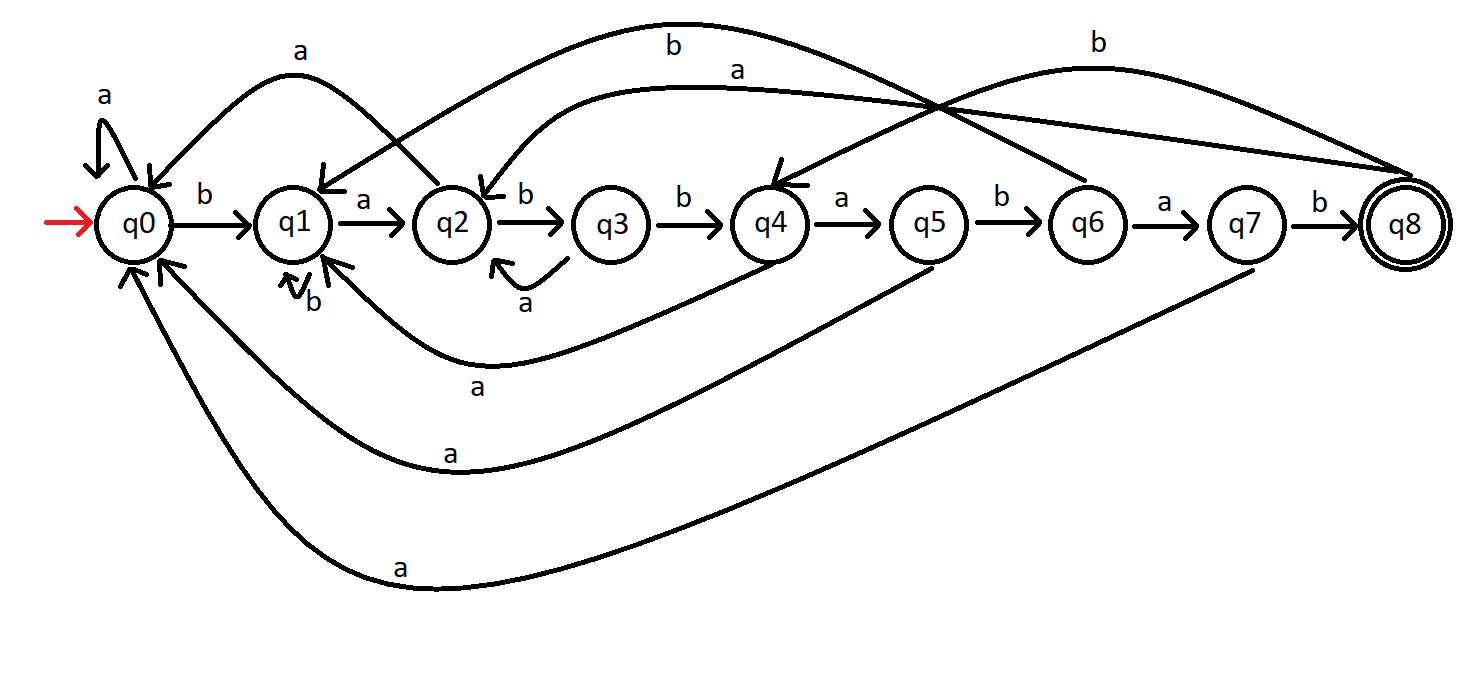
\includegraphics[scale=0.57]{01.png}
\newline\textbf{2)}  
Принимающие состояния: $q_8$, начальное состояние: $q_0$, алвавит = \{a, b, и еще какие-то символы\}, функция переходов и все состояния:

    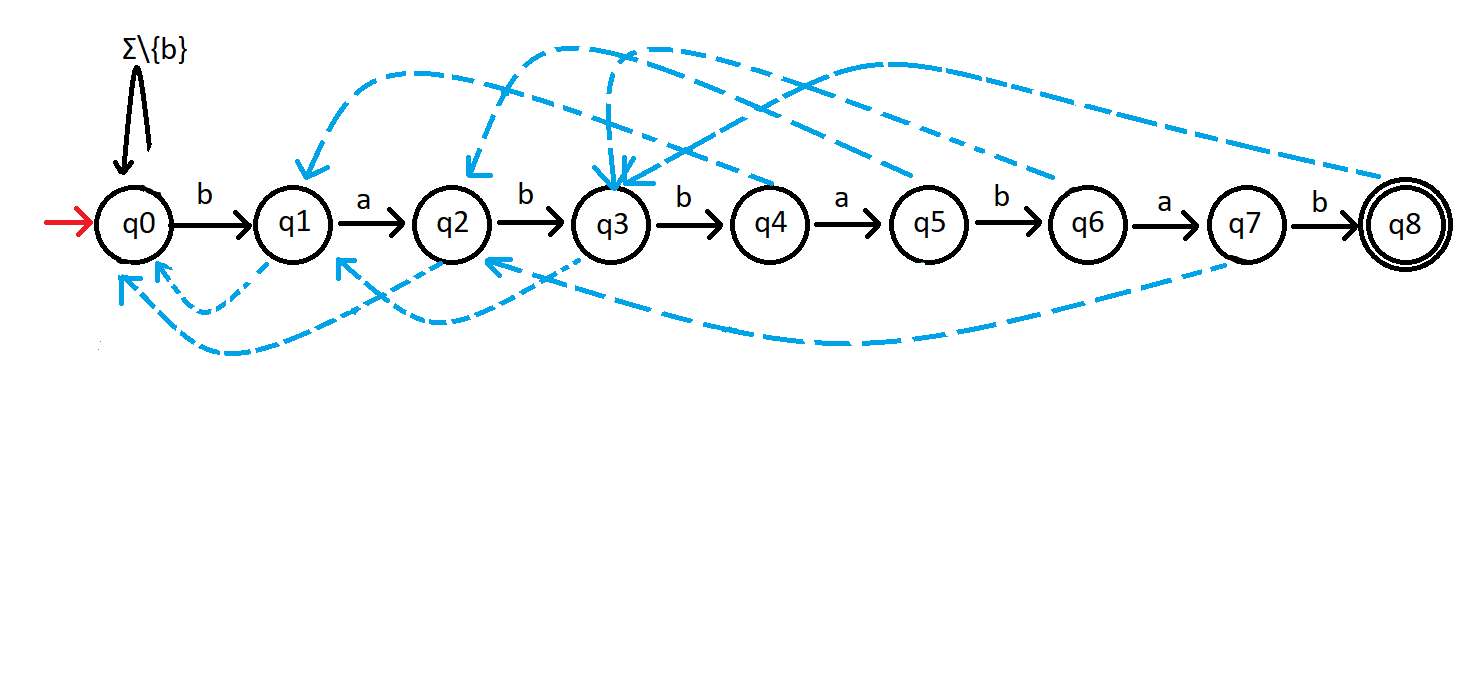
\includegraphics[scale=0.57]{02.png}
\newline\textbf{3)}
$\omega =$ babbabbabab
\begin{enumerate}
    \item Из состояния $q_0$ переходим в состояние $q_1$ по букве b.
    \item Из состояния $q_1$ переходим в состояние $q_2$ по букве a.
    \item Из состояния $q_2$ переходим в состояние $q_3$ по букве b.
    \item Из состояния $q_3$ переходим в состояние $q_4$ по букве b.
    \item Из состояния $q_4$ переходим в состояние $q_5$ по букве a.
    \item Из состояния $q_5$ переходим в состояние $q_6$ по букве b.
    \item Из состояния $q_6$ переходим в состояние $q_3$ по ссылке, переходим в состояние $q_4$ по букве b.
    \item Из состояния $q_4$ переходим в состояние $q_5$ по букве a.
    \item Из состояния $q_5$ переходим в состояние $q_6$ по букве b.
    \item Из состояния $q_6$ переходим в состояние $q_7$ по букве a.
    \item Из состояния $q_7$ переходим в состояние $q_8$ по букве b.
\end{enumerate}
Слово принято, всё отлично.
\newline$\omega = babbabc$
\begin{enumerate}
    \item Из состояния $q_0$ переходим в состояние $q_1$ по букве b.
    \item Из состояния $q_1$ переходим в состояние $q_2$ по букве a.
    \item Из состояния $q_2$ переходим в состояние $q_3$ по букве b.
    \item Из состояния $q_3$ переходим в состояние $q_4$ по букве b.
    \item Из состояния $q_4$ переходим в состояние $q_5$ по букве a.
    \item Из состояния $q_5$ переходим в состояние $q_6$ по букве b.
    \item Из состояния $q_6$ переходим в состояние $q_3$ по ссылке, из состояния $q_3$ переходим в состояние $q_1$ по ссылке, из состония $q_1$ переходим в состояние $q_0$, из состояния $q_0$ переходим по c в состояние $q_0$.
\end{enumerate}
Слово не принято:(
\newpage
\subsection{Задача 2}
ДКА для словаря \{ac, acb, b, ba, c, cbb\}

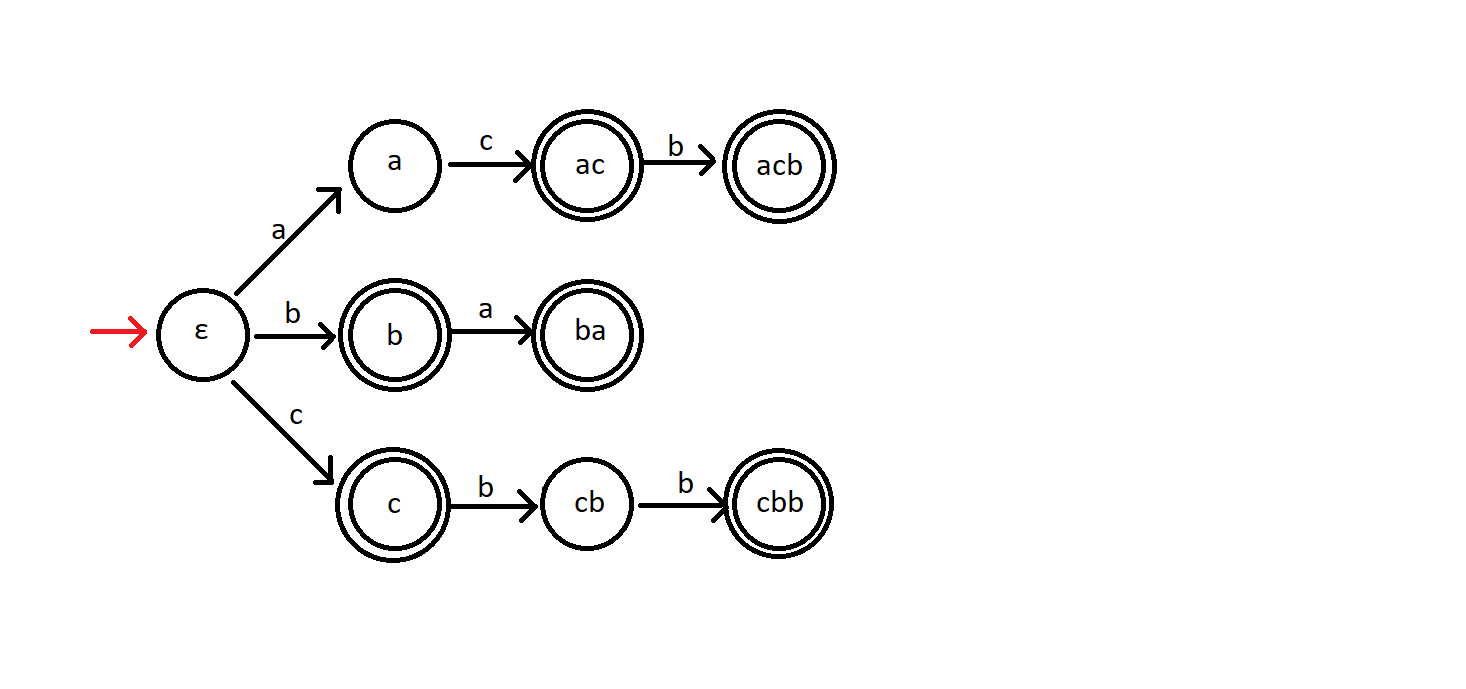
\includegraphics[scale=0.73]{03.png}

ДКА после добавления слова ab в словарь. Добавляем вершину ab и переход из вершины a по букве b.

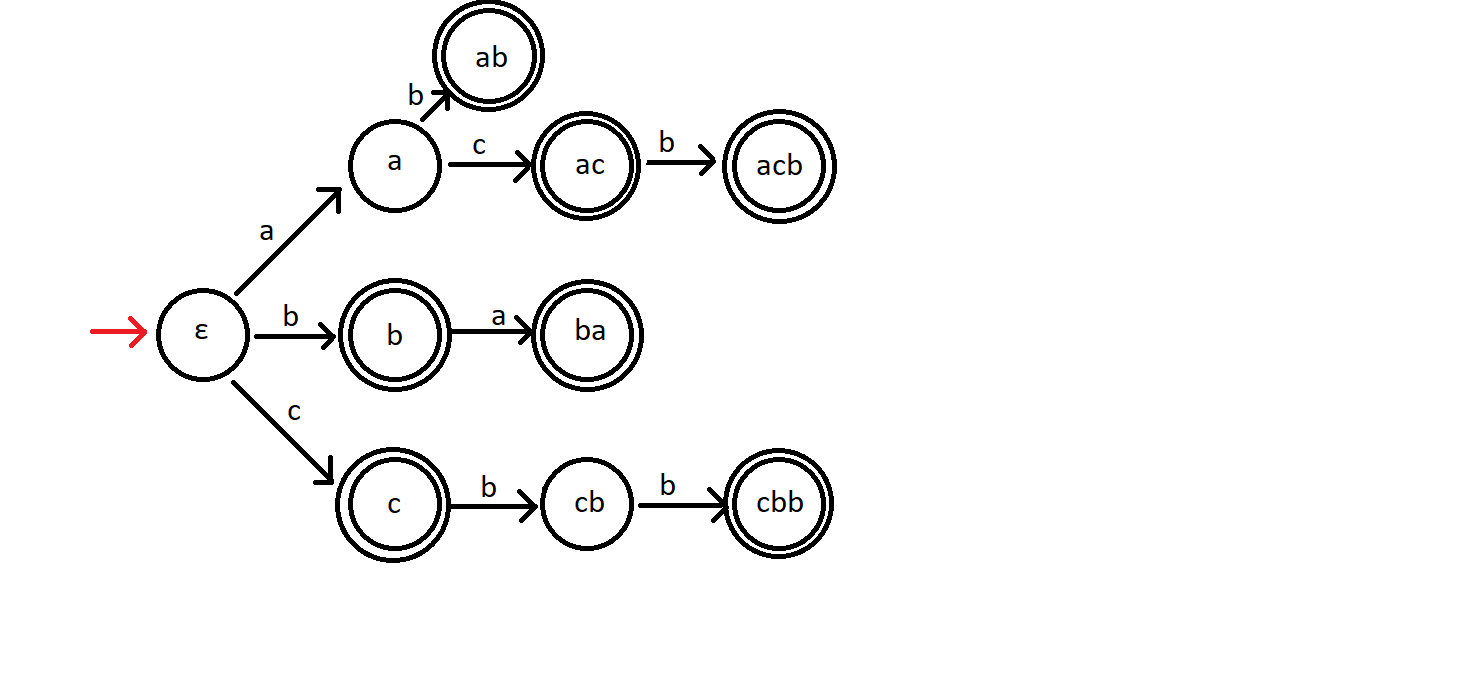
\includegraphics[scale=0.73]{04.png}

ДКА после удаления слова ac из словаря. Больше вершина ac не является принимающим состоянием.

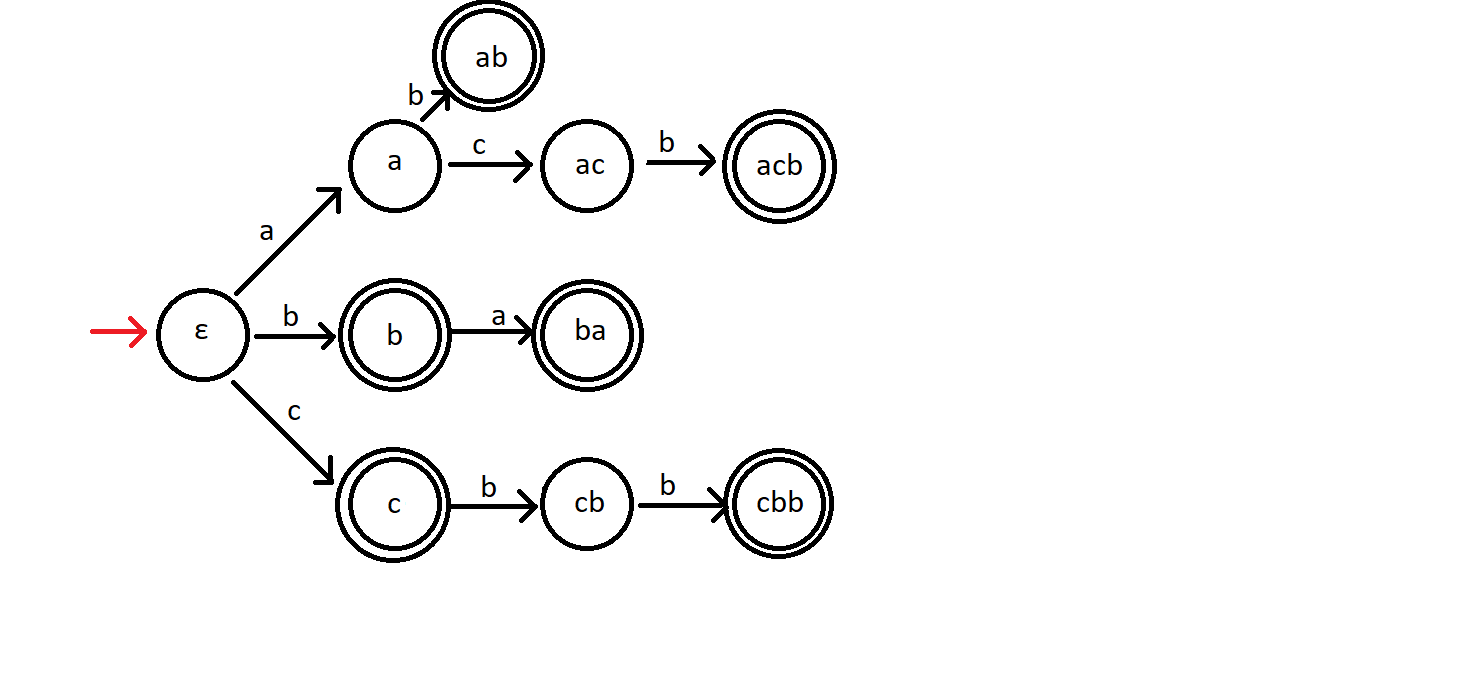
\includegraphics[scale=0.74]{05.png}

\subsection{Задача 3}
Построили автомат Ахо-Карасик для автомата из прошлой задачи. 

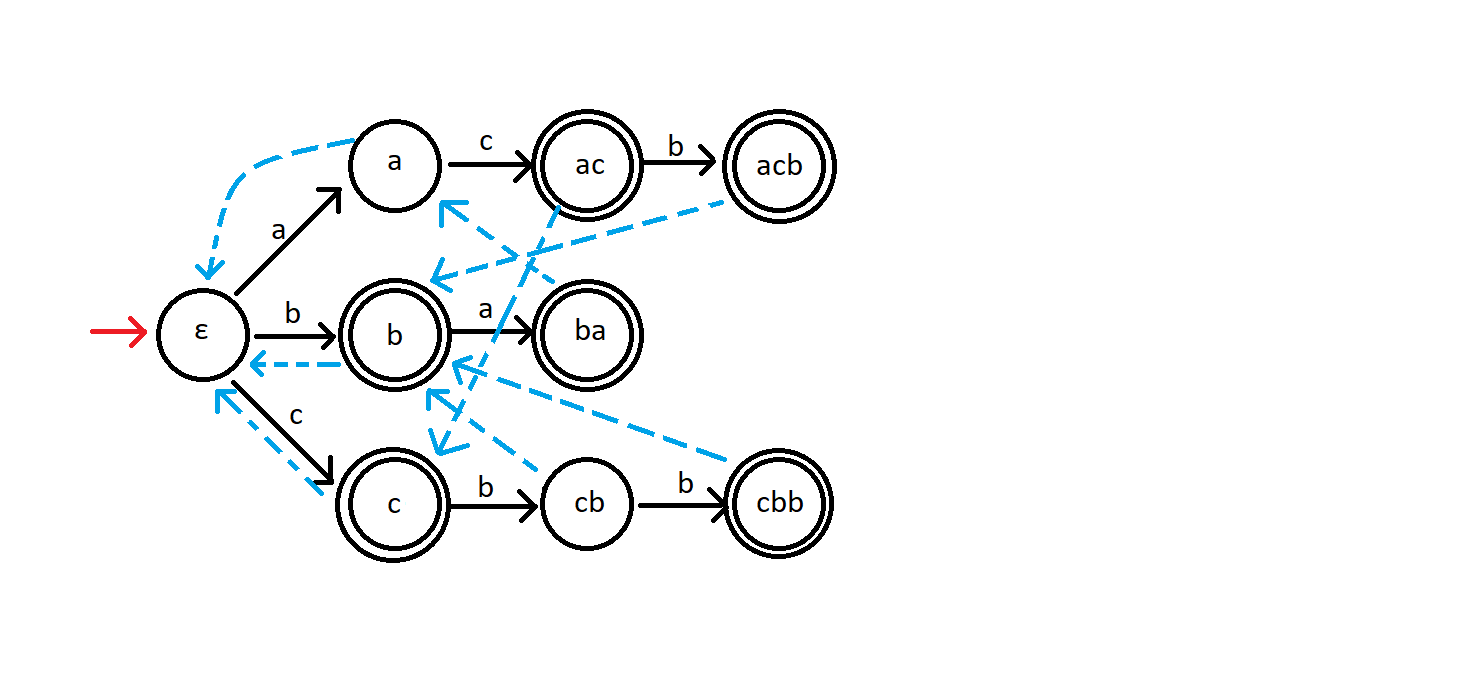
\includegraphics[scale=0.74]{06.png}

$\omega = acbacbb$
\begin{enumerate}
    \item Переходим по букве в состояние a.
    \item Переходим по букве c в состояние ac. 
    (Попали в принимающее состояние, вхождений: 1)
    \item Переходим по букве b в состояние acb.
    (Попали в принимающее состояние, вхождений: 2)
    \item Переходим по ссылке в состояние b, по букве a переходим в состояние ba. 
    (Попали в принимающее состояние, вхождений: 3)
    \item Переходим по ссылке в состояние a, по букве c переходим в состояние ac.
    (Попали в принимающее состояние, вхождений: 4)
    \item Переходим по букве b в состояние acb.
    (Попали в принимающее состояние, вхождений: 5)
    \item Переходим по ссылке в состояние b, потом переходим по ссылке в состояние $\mathcal{E}$, по букве b переходим в состояние b.
    (Попали в принимающее состояние, вхождений: 6)
\end{enumerate}

\subsection{Задача 4}
РВ для этого языка: $\Sigma^{*}a\Sigma^2$

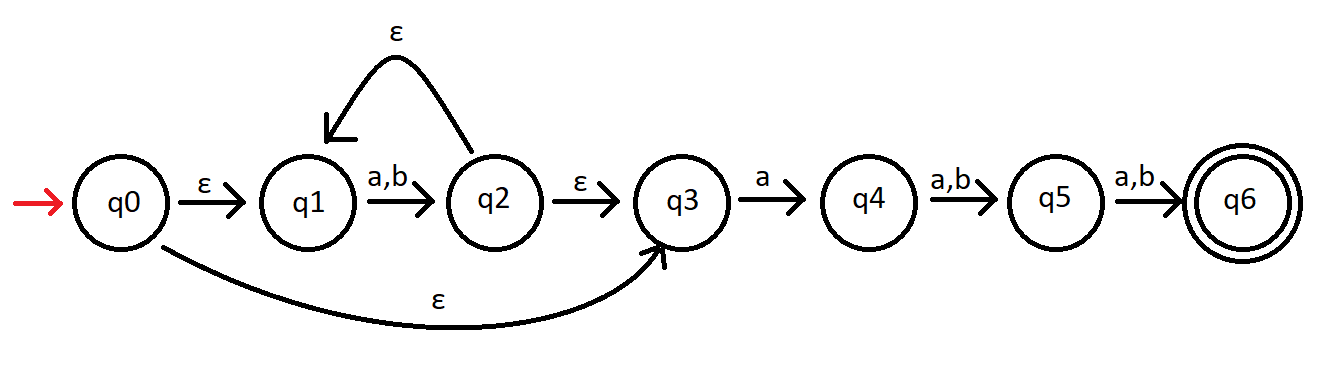
\includegraphics[scale=0.64]{07.png}

    \begin{tabular}{|l|l|l|l|}
    \hline
     & Куда можно перейти & \multicolumn{1}{c|}{a} & \multicolumn{1}{c|}{b} \\ \hline
     $Q_0$ & 1, 3               &  $Q_1$  &  $Q_2$                      \\ \hline
     $Q_1$ & 1, 2, 3, 4         &  $Q_3$  &  $Q_4$                      \\ \hline
     $Q_2$ & 1, 2, 3            &  $Q_1$  &  $Q_2$                      \\ \hline
     $Q_3$ & 1, 2, 3, 4, 5      &  $Q_5$  &  $Q_6$                      \\ \hline
     $Q_4$ & 1, 2, 3, 5         &  $Q_7$  &  $Q_8$                      \\ \hline
     $Q_5$ & 1, 2, 3, 4, 5, 6   &  $Q_5$  &  $Q_6$                      \\ \hline
     $Q_6$ & 1, 2, 3, 5, 6      &  $Q_7$  &  $Q_8$                      \\ \hline
     $Q_7$ & 1, 2, 3, 4, 6      &  $Q_3$  &  $Q_4$                      \\ \hline
     $Q_8$ & 1, 2, 3, 6         &  $Q_1$  &  $Q_2$                      \\ \hline
    \end{tabular}
    $q_i$ эквивалентно i-ому числу.


    Теперь построим автомат по этой картинке, получим такое <<чудо>>.

    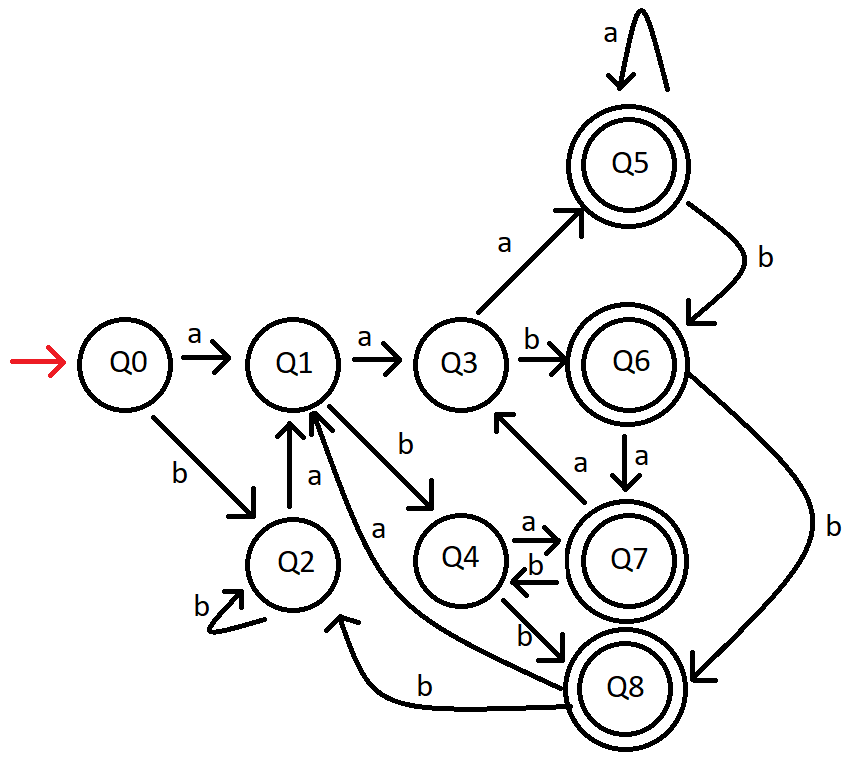
\includegraphics[scale=0.84]{08.png}
\end{document}